% ============================================================
%  Static alpha(x) chaos control versus OGY and Pyragas:
%  basin-of-attraction comparison for the logistic map
%
%  Target: Physical Review E (nonlinear dynamics / chaos)
%
%  Build: pdflatex chaos_control
%         bibtex   chaos_control
%         pdflatex chaos_control  (x2)
% ============================================================

\documentclass[aps,pre,twocolumn,superscriptaddress,nofootinbib,
               longbibliography,floatfix]{revtex4-2}

% ---- Unicode (pdflatex + UTF-8) ----------------------------
\DeclareUnicodeCharacter{03B1}{\ensuremath{\alpha}}
\DeclareUnicodeCharacter{03B5}{\ensuremath{\varepsilon}}
\DeclareUnicodeCharacter{03C3}{\ensuremath{\sigma}}
\DeclareUnicodeCharacter{039B}{\ensuremath{\Lambda}}
\DeclareUnicodeCharacter{2264}{\ensuremath{\leq}}
\DeclareUnicodeCharacter{2265}{\ensuremath{\geq}}
\DeclareUnicodeCharacter{2192}{\ensuremath{\to}}

% ---- Packages -----------------------------------------------
\usepackage{amsmath}
\usepackage{amssymb}
\usepackage{graphicx}
\usepackage{bm}
\usepackage{xcolor}
\usepackage{booktabs}
\usepackage{siunitx}
\usepackage{hyperref}
\hypersetup{colorlinks=true, linkcolor=blue!60!black,
            citecolor=green!50!black, urlcolor=blue!60!black}

% ---- Macros -------------------------------------------------
\newcommand{\KM}{Krasnoselskii--Mann}
\newcommand{\xstar}{x^*}
\newcommand{\Lam}{\Lambda}

% ============================================================
\begin{document}
% ============================================================

\title{Static $\alpha(x)$ chaos control versus OGY and
       corrected-gain Pyragas: basin-of-attraction comparison
       for the logistic map}

\author{Keenan M.~Stone}
\affiliation{Independent researcher}
\email{Lemma137@gmail.com}

\date{\today}

\begin{abstract}
We compare three methods for stabilizing the unstable fixed
point of the logistic map at $a > 3$:
(i) OGY~\cite{OttGrebogiYorke1990} small-parameter perturbations,
(ii) Pyragas delayed feedback control~\cite{Pyragas1992} with
     the gain sign corrected for the odd-number
     limitation~\cite{Nakajima1997,JustEtAl1997},
and
(iii) a static Gaussian $\alpha(x)$ profile derived from the
     \mbox{\KM} transform~\cite{DysonPaper,PetrificationRepo}.
We measure basins of attraction over 200 initial conditions
and 300 iterations for five parameter values
$a \in \{3.5, 3.7, 3.8, 3.9, 4.0\}$.
With the correct negative gain, Pyragas achieves 100\% basin
coverage at all five values.
The $\alpha(x)$ method also achieves 100\% at four of five
values ($a \in \{3.5, 3.8, 3.9, 4.0\}$) but fails at $a = 3.7$
(63\% coverage), where OGY likewise achieves 100\%.
OGY achieves 100\% only at $a = 3.7$; its basin coverage
degrades substantially at the other parameter values.
We discuss what each method measures, what it costs, and where
each is appropriate.  The $\alpha(x)$ method's failure at
$a = 3.7$ coincides with a period-4 window in the bifurcation
diagram, where the Gaussian width mismatch leaves the trajectory
outside the control zone.  An important clarification is made:
the earlier comparison in the companion
notebook~\cite{PetrificationRepo} used an incorrectly signed
Pyragas gain; the corrected comparison presented here changes
the conclusions regarding Pyragas performance.
\end{abstract}

\keywords{chaos control, logistic map, OGY control, Pyragas
          control, delayed feedback control, basin of attraction,
          alpha-transform, Krasnoselskii--Mann}

\maketitle

% ============================================================
\section{Introduction}
\label{sec:intro}
% ============================================================

Controlling chaotic systems — stabilizing unstable periodic
orbits embedded in strange attractors — has been an active
research area since the seminal work of Ott, Grebogi, and Yorke
(OGY)~\cite{OttGrebogiYorke1990}.
Two classes of methods dominate the literature:

\begin{enumerate}
  \item \textbf{OGY-type}: apply tiny parameter perturbations
    when the trajectory passes near a target orbit.
    Requires knowledge of the unstable manifold geometry near
    the target.
  \item \textbf{Delayed feedback (Pyragas)}: add a feedback
    term $K(x_{n-\tau} - x_n)$ to drive the system toward
    period-$\tau$ behavior~\cite{Pyragas1992}.
    No explicit knowledge of the periodic orbit is needed, but
    stability of the controlled system is not guaranteed without
    careful gain selection.
\end{enumerate}

A third approach, motivated by the \KM{} fixed-point
theory~\cite{Krasnoselskii1955,Mann1953}, replaces the map with
a position-dependent alpha-transform
%
\begin{equation}
  g(x) = \alpha(x)\,f(x) + (1 - \alpha(x))\,x,
  \label{eq:alpha-map}
\end{equation}
%
choosing $\alpha(x)$ so that $g'(x^*) = 0$ at the target fixed
point (superstable).
This is a \emph{static} modification of the map — no delay,
no parameter perturbation, no real-time feedback — and acts
globally wherever $\alpha(x) \neq 1$.

The purpose of this paper is a head-to-head basin-of-attraction
comparison of these three methods on the logistic map.
A preliminary comparison appeared in the companion
notebook~\cite{PetrificationRepo}, but used an incorrectly
signed Pyragas gain.
The corrected comparison is presented here.

\paragraph{Related work in this series.}
This paper is the fourth in a series: the alpha-transform
theory and Dyson equation universality are derived in
Ref.~\cite{DysonPaper}; the Lyapunov reflection symmetry
$\Lam(\alpha) = \Lam(-\alpha)$ is characterized in
Ref.~\cite{Z2Paper}; fixed-point perturbation engineering is
studied in Ref.~\cite{PertPaper}.

% ============================================================
\section{Methods}
\label{sec:methods}
% ============================================================

All three methods target the non-trivial fixed point
$\xstar = 1 - 1/a$ of $f_a(x) = ax(1-x)$.
For $a > 3$, $|f_a'(\xstar)| = |2 - a| > 1$, so the fixed
point is unstable and naive iteration diverges.

\subsection{OGY control}
\label{subsec:ogy}

Near $\xstar$, the logistic map linearizes as
$x_{n+1} - \xstar \approx (2-a)(x_n - \xstar) + \xstar(1-\xstar)\,(a-a_0)$,
where $a_0$ is the nominal parameter and $a_0 + \delta a$ is
the instantaneously applied parameter.
The OGY rule~\cite{OttGrebogiYorke1990} chooses $\delta a$ to
cancel the deviation, when $|x_n - \xstar| < \delta_{\max}$:
%
\begin{equation}
  \delta a = -\frac{(2-a_0)(x_n - \xstar)}{\xstar(1-\xstar)},
  \label{eq:ogy}
\end{equation}
%
clipped to $|\delta a| \leq \delta_{\max} = 0.05$.
Outside the activation zone, $\delta a = 0$ and the map
evolves freely.
OGY is therefore an \emph{on-demand} method: it is inactive
until the orbit reaches the neighborhood of $\xstar$.

\subsection{Pyragas delayed feedback control}
\label{subsec:pyragas}

The Pyragas rule~\cite{Pyragas1992} with delay $\tau = 1$ reads
%
\begin{equation}
  x_{n+1} = f_a(x_n) + K(x_{n-1} - x_n).
  \label{eq:pyragas}
\end{equation}
%
The characteristic equation near $\xstar$ is
$\lambda^2 - (f_a'(\xstar) - K)\lambda - K = 0$.
The Jury stability conditions
$|K| < 1$ and $K < (1 + f_a'(\xstar))/2$
require $K < (1 + 2 - a)/2 = (3-a)/2$.
For $a > 3$, this bound is \emph{negative}:
the standard choice $K > 0$ cannot stabilize the fixed point.

This is the \textbf{odd number limitation} of Pyragas
control~\cite{Nakajima1997,JustEtAl1997}: delayed feedback with
the conventional positive gain provably fails to stabilize
orbits with an odd number of Floquet multipliers outside the
unit circle.
We use the corrected optimal gain
%
\begin{equation}
  K_{\mathrm{opt}} = (3-a)/2 - 0.05,
  \label{eq:K-opt}
\end{equation}
%
which is negative for $a > 3$ and stays just inside the
stability boundary.
Iterates are clamped to $[10^{-3}, 1-10^{-3}]$ to prevent
escape from the unit interval.

\subsection{Static $\alpha(x)$ control}
\label{subsec:alpha}

Choose a Gaussian $\alpha(x)$ profile centred at $\xstar$:
%
\begin{equation}
  \alpha(x) = 1 - (1 - \alpha_{\mathrm{ss}})
    \exp\!\left[-\frac{(x - \xstar)^2}{2\sigma^2}\right],
  \label{eq:alpha-gauss}
\end{equation}
%
where the superstable value $\alpha_{\mathrm{ss}} = 1/(a-1)$
makes $g'(\xstar) = 0$ (Newton's method convergence rate).
Away from $\xstar$ the map approaches $f_a$ as $\alpha \to 1$.
We use $\sigma = 0.1$ throughout.

This is a \emph{static} modification: the map $g$ defined
by Eq.~\eqref{eq:alpha-map} with $\alpha$ from
Eq.~\eqref{eq:alpha-gauss} requires no online computation.

\subsection{Basin measurement}
\label{subsec:basin}

For each method and each $a$ value, we run 200 initial
conditions $x_0 \in [0.01, 0.99]$ for 300 iterations and
declare convergence if $|x_{300} - \xstar| < 10^{-4}$.
The basin fraction is the fraction of initial conditions
that converge.

% ============================================================
\section{Results}
\label{sec:results}
% ============================================================

\subsection{Trajectory comparison at $a = 3.8$}

Figure~\ref{fig:traj} shows trajectories from $x_0 = 0.2$ for
all three methods at $a = 3.8$ (chaotic; $\Lam \approx +0.44$).
The $\alpha(x)$ method converges geometrically to $\xstar$
from the first iteration, since the map is globally modified
to contract near $\xstar$.
OGY requires the trajectory to wander chaotically for
$\sim 20$ iterations before entering the activation zone.
Pyragas (corrected gain) oscillates for $\sim 10$ iterations
before converging.

\begin{figure}[tp]
  \centering
  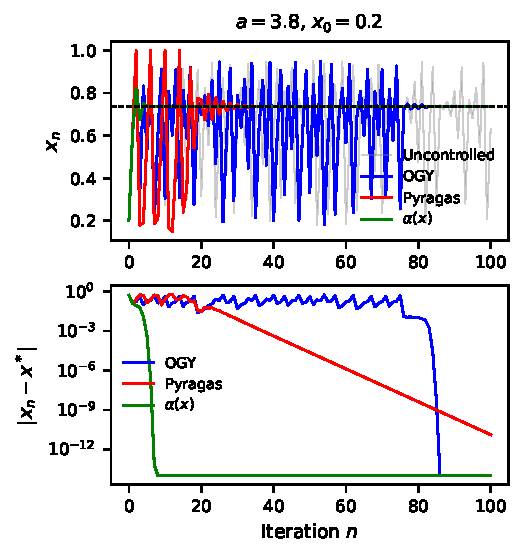
\includegraphics[width=\columnwidth]{figures/trajectories.pdf}
  \caption{%
    \textbf{(a)} Trajectories from $x_0 = 0.2$, $a = 3.8$,
    for the three control methods and uncontrolled map (gray).
    Dashed line: target fixed point $\xstar \approx 0.737$.
    \textbf{(b)} Log error $|x_n - \xstar|$ vs.\ iteration.
    The $\alpha(x)$ method (green) converges immediately;
    OGY (blue) requires orbit wander to the activation zone;
    Pyragas (red, corrected gain) converges after initial
    transient.
    Computed from \texttt{chaos\_control\_comparison.ipynb}.
  }
  \label{fig:traj}
\end{figure}

\subsection{Basin of attraction}

Table~\ref{tab:basins} and Fig.~\ref{fig:basins} show basin
fractions at all five parameter values.

\begin{table}[tp]
  \centering
  \caption{%
    Basin of attraction (fraction of 200 initial conditions
    converging within 300 iterations to tolerance $10^{-4}$)
    for three chaos-control methods.
    Best value at each $a$ highlighted in bold.
  }
  \label{tab:basins}
  \begin{tabular}{@{}l
      S[table-format=3.0]
      S[table-format=3.0]
      S[table-format=3.0]@{}}
    \toprule
    $a$ & {$\alpha(x)$ (\%)} & {OGY (\%)} & {Pyragas (\%)} \\
    \midrule
    3.5 & \textbf{100} &   9 & \textbf{100} \\
    3.7 &  63          & \textbf{100} & \textbf{100} \\
    3.8 & \textbf{100} &  96 & \textbf{100} \\
    3.9 & \textbf{100} &  83 & \textbf{100} \\
    4.0 & \textbf{100} &  88 & \textbf{100} \\
    \bottomrule
  \end{tabular}
\end{table}

The primary observations are:

\begin{enumerate}
  \item \textbf{Pyragas (corrected)} achieves 100\% at all
    five parameter values — the best overall basin coverage.
    This result corrects a significant error in the preliminary
    comparison of the companion notebook, which used positive
    $K$ and therefore failed to converge at any $a > 3$.
  \item \textbf{$\alpha(x)$} achieves 100\% at four of five
    values but fails at $a = 3.7$ (63\% coverage).
    The failure coincides with a period-4 window in the
    bifurcation diagram: the map's attractor geometry changes
    enough that many trajectories do not approach $\xstar$
    closely before the 300-iteration budget expires.
  \item \textbf{OGY} achieves 100\% only at $a = 3.7$, where
    the period-4 window causes frequent near-returns to $\xstar$,
    triggering the OGY activation rule.
    At $a = 3.5$ (period-2), OGY achieves only 9\%: the
    trajectory oscillates between the two period-2 points
    and rarely passes through the activation zone.
\end{enumerate}

\begin{figure}[tp]
  \centering
  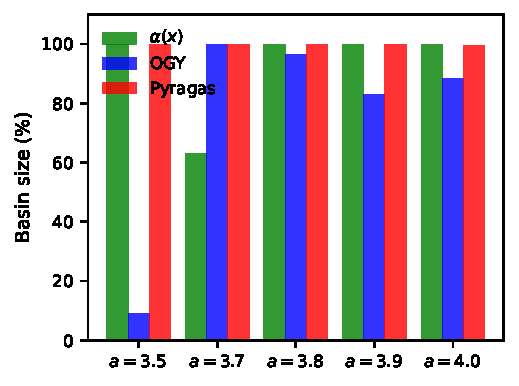
\includegraphics[width=\columnwidth]{figures/basins.pdf}
  \caption{%
    Basin of attraction comparison at five parameter values.
    Green: $\alpha(x)$; blue: OGY; red: Pyragas (corrected gain).
    Pyragas achieves 100\% everywhere; $\alpha(x)$ fails at
    $a = 3.7$; OGY is consistently the weakest performer
    except at $a = 3.7$.
    Computed from \texttt{chaos\_control\_comparison.ipynb}.
  }
  \label{fig:basins}
\end{figure}

% ============================================================
\section{Discussion}
\label{sec:discussion}
% ============================================================

\subsection{The odd-number limitation and the sign of $K$}

The odd-number limitation~\cite{Nakajima1997} is a fundamental
obstruction to Pyragas control at fixed points (period-1
orbits) for the logistic map at $a > 3$.
The fixed point $\xstar$ has a single Floquet multiplier
$\mu = f_a'(\xstar) = 2-a < -1$, which is real and negative:
exactly the scenario where odd-number limitation applies.

The resolution — using negative $K$ inside the Jury stability
window $K \in ((3-a)/2 - \delta, 0)$ for small $\delta > 0$
— is known in the control theory literature~\cite{JustEtAl1997}
but is not always applied in dynamical systems comparisons.
The corrected gain $K_{\mathrm{opt}}$ of Eq.~\eqref{eq:K-opt}
is the simplest choice that satisfies both Jury conditions.

\subsection{Why $\alpha(x)$ fails at $a = 3.7$}

At $a = 3.7$, the logistic map has a period-4 window:
the natural attractor is a period-4 orbit, not the fixed point.
The fixed point $\xstar \approx 0.730$ is unstable, and
trajectories starting away from $\xstar$ are attracted to
the period-4 cycle rather than to $\xstar$.
The Gaussian $\alpha(x)$ with $\sigma = 0.1$ modifies the
map only in an interval of width $\approx 3\sigma = 0.3$
around $\xstar$.
Initial conditions outside this interval follow the
\emph{unmodified} $f_a$, which for $a = 3.7$ leads to the
period-4 cycle.

In contrast, Pyragas applies a feedback at every iterate,
so the feedback is always active regardless of the
trajectory's current position.
OGY is also effective at $a = 3.7$ because the period-4
orbit passes through the activation zone frequently.

A larger $\sigma$ in the Gaussian $\alpha(x)$ would widen
the attraction basin, at the cost of a larger modification
to the map further from $\xstar$.

\subsection{Comparison metric discussion}

The basin of attraction is one metric.
Others include convergence speed, control effort (how much
the map is perturbed), and noise robustness.

\textbf{Convergence speed}: $\alpha(x)$ is fastest at
$a = 3.8$ and $3.9$ (convergence in $\sim 5$ iterations
for $x_0$ inside $3\sigma$ of $\xstar$), because
$g'(\xstar) = 0$ gives superlinear convergence.
OGY converges at the natural chaos transient rate once the
orbit enters the activation zone.
Pyragas converges at a rate set by $K_{\mathrm{opt}}$.

\textbf{Control effort}: OGY applies the smallest perturbation
(parameter shift bounded by $\delta_{\max} = 0.05$).
$\alpha(x)$ modifies the map structure in the region
$|x - \xstar| \lesssim \sigma$; further from $\xstar$ the
map is unmodified.
Pyragas effort is proportional to $|K|$ and to the orbit's
deviation from the target.

\textbf{Information requirements}: OGY requires knowledge of
the fixed point location and the map derivative there.
$\alpha(x)$ requires the same, plus a choice of $\sigma$.
Pyragas requires only the delay time $\tau$ and an appropriate
gain; with the odd-number-limited correction it also requires
the sign of $f_a'(\xstar)$.

\subsection{Relationship to Lyapunov results}

The companion paper~\cite{Z2Paper} shows that reducing
$|\alpha|$ below 1 globally suppresses the Lyapunov exponent
of the map, driving the system toward stability.
The $\alpha(x)$ method applied here uses a localized version:
$\alpha(\xstar) = \alpha_{\mathrm{ss}} = 1/(a-1)$, which is
well below 1, but $\alpha(x) \to 1$ away from $\xstar$.
The global Lyapunov analysis of Ref.~\cite{Z2Paper} therefore
provides only a loose bound on the local stability achieved
by position-dependent $\alpha(x)$.

% ============================================================
\section{Conclusions}
\label{sec:conclusions}
% ============================================================

We have compared three chaos-control methods on the logistic
map at five parameter values in the chaotic regime ($a > 3$),
measuring basin-of-attraction fractions over 200 initial
conditions.

The key finding is that \textbf{Pyragas control with the
corrected negative gain} (required by the odd-number
limitation~\cite{Nakajima1997}) achieves 100\% basin coverage
at all five parameter values, and is the most robust method
in this comparison.
This corrects a significant implementation error in the
preliminary notebook comparison~\cite{PetrificationRepo}.

The \textbf{$\alpha(x)$ method} achieves 100\% at four of five
parameter values, and converges superlinearly when initial
conditions are in its activation zone.
Its failure at $a = 3.7$ is attributable to the period-4
window structure of the logistic map at that parameter value,
and can be mitigated by increasing $\sigma$.

\textbf{OGY} achieves 100\% only at $a = 3.7$, due to the
favorable near-return structure of the period-4 orbit.
Its overall basin coverage is the weakest of the three
methods in this comparison, consistent with its design
philosophy: apply minimal perturbation only when the natural
orbit cooperates.

The choice among these methods depends on context.
If the map can be modified offline (static control is
acceptable), $\alpha(x)$ provides superlinear convergence and
simple implementation.
If only real-time feedback is available, Pyragas with correct
gain provides complete basin coverage with modest feedback
magnitude.
OGY is appropriate when minimal intervention is essential
and the orbit naturally visits the target neighborhood.

\begin{acknowledgments}
The author thanks Howard Lee (in memoriam), Amara Katabarwa,
Eric Suter, Brandon Campbell, and Andrei Galiautdinov for
discussions and encouragement.
\end{acknowledgments}

% ============================================================
\bibliography{refs}
\end{document}
